\part{Historisk Utvikling}
\chapter{Bruddet med Klassisk Fysikk}
\section{Hva er Kvantemekanikk?} 
Kvantemekanikk forsøker å beskrive fysiske systemer på kvante nivå. Her står Schrödinger's likning sentralt. 

\subsection{Energikvantisering}
Energi i Kvantemekanikken er ikke en kontinuerlig størrelse. Den har diskrée verdier. Dette kalles energikvantisering. Dette gjelder både fotoner og elektroner. 

\subsection{Bølge-Partikkel-dualitet}
Vi vet ikke helt hva er partikkel er, men det vi vet er at de har egenskaper som minner om partikler og bølger. Dette kalles bølge-partikkel-dualiteten. Vi kan skyte ut fotoner i små energi pakker eller kvanter hvor de vil oppføre seg som partikler, men som en ser i dobbelspalteeksperimentet kan de likevel oppføre seg som bølger på samme tid. Da trenger vi Schrödinger's bølgeligning.

\subsection{Egentilstand og superposisjon}
En partikkel med kvantisert energien $ ϵ_{n} $ befinner seg i en tilstand som er beskrevet av bølgefunksjonen $ ψ_{n} $. Dette kalles en energi-egentilstand. En partikkel kan være i flere energi-egentilstander samtidig. Dette kalles superposisjon. Vi kan tenke på Schrödinger's katt som en partikkel som er i en superposisjon av to energi-egentilstander, død og levende. Da får vi følgende:
\[
ψ = c_{\text{død}} ⋅ ψ_{\text{død}} + c_{\text{levende}} ⋅ ψ_{\text{levende}}
\]
Hvis vi måler tilstanden til katten vil vi få én av de to tilstandene. Enten død eller levende. Da ender vi opp i det som kalles \textit{egentilstand} fra bølgefunksjonen/superposisjon. Sannsynligheten for at katten er død er da $ \left\vert c_{\text{død}} \right\vert ^{2} $ og Sannsynligheten for at katten er levende er $ \left\vert c_{\text{levende}} \right\vert ^{2} $. Det eneste Kvantemekanikken kan fortelle oss er sannsynligheten for at katten er i en tilstand, ikke om den er i den tilstanden eller ikke, før vi måler det. 

\subsection{Heisenberg's uskarphetsrelasjon}
I klassisk mekanikk er foreksempel posisjon $ \mathbf{x} $ og bevegelsesmengde $ \mathbf{p} $ uavhengig størrelser. I Kvantemekanikken impliserer via Heisenberg's uskarphetsrelasjon at en ikke kan observerer begge til en vilkårlig presisjon. Dette uttrykkes via følgende formel
\[
Δ \mathbf{p} Δ\mathbf{x} \geq \frac{ℏ}{2}
\]
hvor $ Δ\mathbf{x} $ er usikkerheten i posisjon og $ Δ\mathbf{p} 
$ er usikkerheten i bevegelsesmengde. Dette er bare en merkbart på atomært nivå, men gjelder teknisk sett alltid. 

\subsection{Paulis eksklusjonsprinsipp}
To fermioner (f.eks elektroner, protoner, kvarker og nøytrinoer) akn ikke befinne seg i samme tilstand (dvs. samme energi samme sted). Dette ser vi i atomer hvor elektronene fyller opp skall slik at nye elektroner må fylle opp et nytt skall. 



\section{Enheter i Kvantefysikk}
\subsection{Lengde}
For å unngå ekstremt små eller store tall bruker vi litt smarte enheter. Kvantefysikken operer på størrelser fra $ 10^{-8} $ til $ 10^{18} $m. Nanometer (nm) er $ 10^{-9} $m, femtometer (fm) er $ 10^{-15} $m og ångstrøm (Å) er $ 10^{-10} $m / $ 0.1 $nm.

\subsection{Energi}
For energi brukes til vanlig Joule, men energien i kvantemekanikken er så liten som $ 10^{-19} $J. Da bruker vi eV (elektronvolt) som er $ 1.602 \cdot 10^{-19} $C. Dette kommer fra at 1J er likt med 1C $\cdot$ 1V. Da er 1 eV den kinetiske energien et elektron får når den akselereres gjennom en potensialdifferensen på 1V. 

\subsection{Masse}

Istedet for å bruke kg for å måle masse kan vi heller bruke MeV/c$^{2}$. Dette kommer fra likningen $ E = mc^{2} $. Ser vi på hvileenergien til med enheten eV får vi 
\[
E_{0}^{\text{elektron}} = m_{e} c^{2} = 5.11 \cdot 10^{5} \text{eV}
\]
Løser vi dette for massen $ m_{e} $ får vi
\[
m_e = E_{0}^{\text{elektron}} / c^{2} = 0.511\ \text{MeV}/c^{2}
\]

\subsection{Andre Konstanter}
\textbf{Placks konstant}
\[
h = 6.626 ⋅  10^{-34} \text{ Js} = 4.135 ⋅ 10^{-15} \text{  eVs}
\]
\[
ℏ = \frac{h}{2 \pi} = 1.055 ⋅ 10^{-34} \text{Js} = 6.582 ⋅ 10^{-16} \text{eVs} 
\]
\[
hc = 1240 \text{ eV nm} (\text{MeV fm})
\]
\[
ℏc = 197.3 \text{ eV nm} (\text{MeV fm})
\]
Noen ganger kan det lønne seg å gange en brøk med $ c $ oppe og nede for å få inn konstanten $ ℏc $. Utrykket under hadde medført veldig små størrelser ($ 10^{-34} $ og $ 10^{-31} $) og dermed ville det blitt vanskelig å regne med. 
\[
\frac{h}{m_e c} = \frac{hc}{m_e c^{2}} = \frac{1240 \text{eV nm}}{0.511 ⋅ 10^{6}} ≈ 0.002 nm
\]
\subsection{Coulomb-potensialet}
\[
V(r) = \frac{e^{2}}{4 \pi \epsilon_{0} r} = \frac{k_e e^{2}}{2}, \qquad k_e e^{2} = 1.44 \text{eV nm}
\]
\subsection{Nyttige Tabeller}

\begin{figure}[ht!]
  \centering
  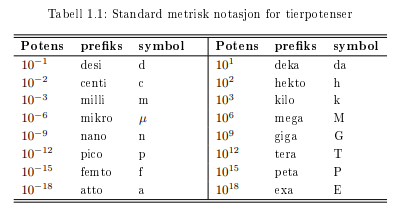
\includegraphics[scale = 1]{Figures/Metric power notation .png}
  \caption{}
  \label{fig: Metric power notation}
\end{figure}

\begin{figure}[ht!]
  \centering
  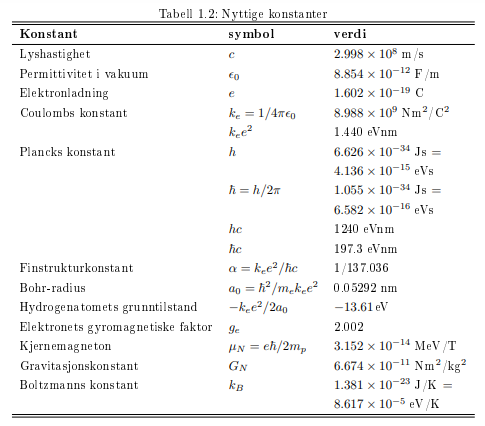
\includegraphics[scale = 1]{Figures/Constants table.png}
  \caption{}
  \label{fig: Constants table}
\end{figure}

\begin{figure}[ht!]
  \centering
  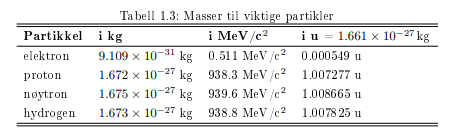
\includegraphics[scale = 1]{Figures/Masser til viktige partikler.png}
  \caption{}
  \label{fig: Masser til viktige partikler}
\end{figure}

\begin{figure}[ht!]
  \centering
  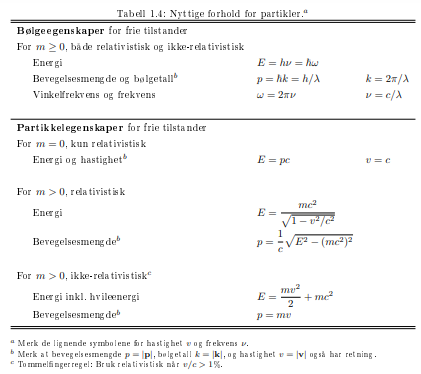
\includegraphics[scale = 1]{Figures/Nyttige forhold for partikler.png}
  \caption{}
  \label{fig: Nyttige forhold for partikler}
\end{figure}

